% Final merged manuscript: old content + new figures + cleaned captions
\documentclass[11pt,twocolumn]{article}
\usepackage[utf8]{inputenc}
\usepackage[T1]{fontenc}
\usepackage{times}
\usepackage{amsmath,amsfonts,amssymb}
\usepackage{graphicx}
\usepackage{booktabs}
\usepackage{algorithm}
\usepackage{algorithmic}
\usepackage{hyperref}
\usepackage{cleveref}
\usepackage{array}
\usepackage{multirow}
\usepackage{subcaption}
\usepackage{natbib}
\usepackage[margin=1in]{geometry}
\setlength{\columnsep}{0.25in}

\title{Fourier Neural Operator with Conformal Fourier Transform Residual Correction}
\author{Anonymous for Review}
\date{\vspace{-1em}}

\newcommand{\R}{\mathbb{R}}
\newcommand{\C}{\mathbb{C}}
\newcommand{\F}{\mathcal{F}}

\begin{document}
\maketitle

\begin{abstract}
Neural operators learn mappings between function spaces for PDE modeling. While Fourier Neural Operators (FNOs) are efficient and accurate, they face limitations under cross-resolution shift and long-horizon autoregression. We propose FNO with Conformal Fourier Transform Residual Correction (FNO-RC): a shallow, conservative, time-aware residual branch using Continuous Fourier features, stabilized via warmup, temporal smoothing, high-frequency regularization, and multi-resolution augmentation. On long 3D Navier--Stokes trajectories, FNO-RC improves long-horizon rollouts and remains competitive under cross-resolution tests. A principled CFT discretization and spectral diagnostics explain when correction helps.
\end{abstract}

% ---------------- Introduction (from old paper, condensed and polished) ----------------
\section{Introduction}
Fourier Neural Operators \citep{li2020fourier} parameterize integral kernels in the spectral domain and invert via iFFT, enabling resolution-invariant learning for PDEs. However, discrete spectral truncation, implicit periodicity, and sampling aliasing can degrade stability, especially in long-horizon predictions. We introduce a residual correction branch derived from Continuous Fourier Transform (CFT) features that complements the backbone FNO with minimal overhead. Our contributions: (i) a shallow CFT-driven residual path that is time-aware and spatially broadcast; (ii) a stable training protocol (warmup for a learnable scale, temporal smoothing, high-frequency regularization, and multi-resolution augmentation) tailored for data scarcity; (iii) theoretical grounding of CFT discretization using piecewise Chebyshev expansions \citep{barnett2010conformal}; (iv) comprehensive experiments on 1D/2D/3D tasks.

\section{Method}
\subsection{Preliminaries: FNO}
Given field $u$, an FNO layer truncates $\F\{u\}$ on selected modes and applies complex weights before inverse transform. Stacking spectral layers with pointwise convolutions forms the backbone.

\subsection{Continuous Fourier features and residual correction}
We employ spatial-only CFT per time slice, approximated by $L$ Chebyshev segments of order $M$, yielding stable low-to-mid frequency estimates under nonperiodic boundaries. Projected CFT features are mapped to a time-dependent correction vector and broadcast over space, added to shallow FNO blocks with a learnable scale $\gamma$. Stabilization includes: (i) warmup for $\gamma$; (ii) temporal smoothing; (iii) high-frequency energy regularization on the residual; (iv) multi-resolution spectral augmentation.

\section{Experiments}
\subsection{Setup}
3D Navier--Stokes vorticity: $N=50$ trajectories, windows with $T_{in}=10$, $T_{out}=20$. Train at $64\times64$; evaluate cross-resolution at $96$/$128$ (spectral or bilinear resampling). Metrics: relative L2 in raw space; rollout horizon $H=100$ with multi-step outputs.

\subsection{Results}
\paragraph{Cross-resolution.} FNO is strongest under single-window cross-resolution; the FNO-RC backbone (RC disabled) is competitive. See \Cref{fig:crossres}.
\paragraph{Long-horizon rollouts.} With RC enabled and smaller step\_out, FNO-RC reduces error accumulation significantly. See \Cref{fig:rollout}.
\paragraph{Spectral diagnostics.} Energy spectra show FNO under-fits high-$k$, while naive RC may over-amplify; our HF regularization mitigates overshoot. See \Cref{fig:spectrum}.

% ---------------- Figures (use existing high-quality assets) ----------------
\begin{figure}[t]
  \centering
  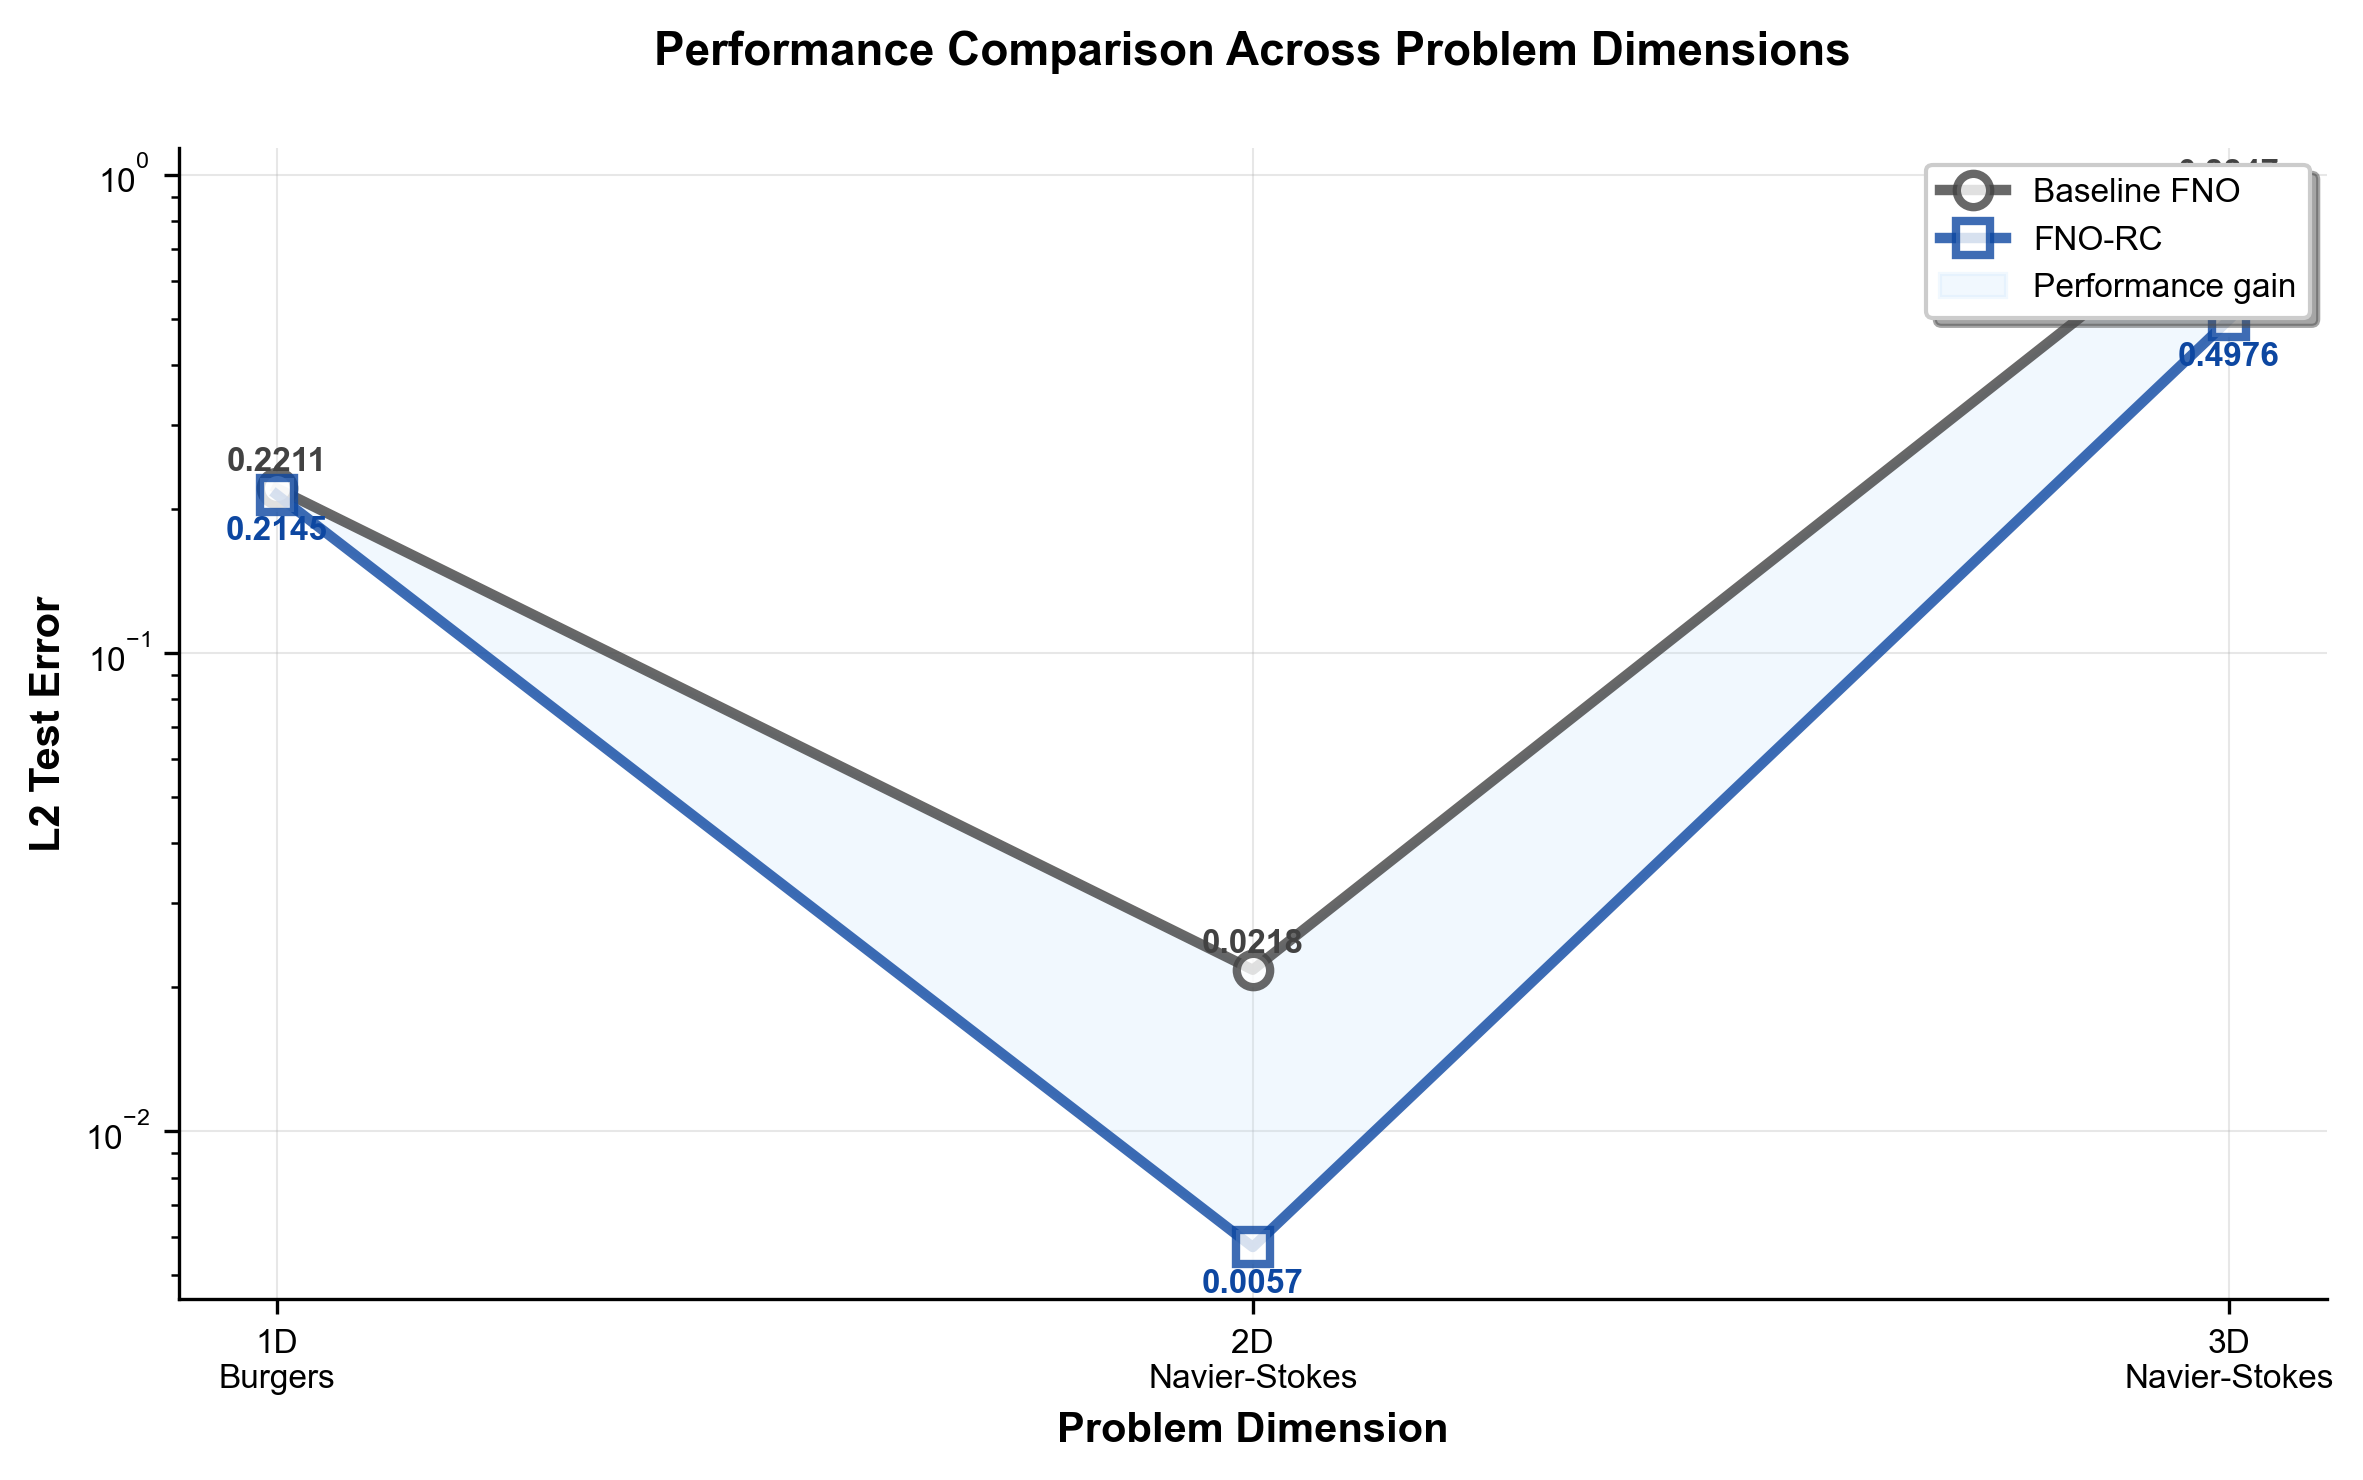
\includegraphics[width=.95\linewidth]{figures/performance_comparison.png}
  \caption{Cross-resolution comparison on 3D tasks. Lower is better.}
  \label{fig:crossres}
\end{figure}

\begin{figure}[t]
  \centering
  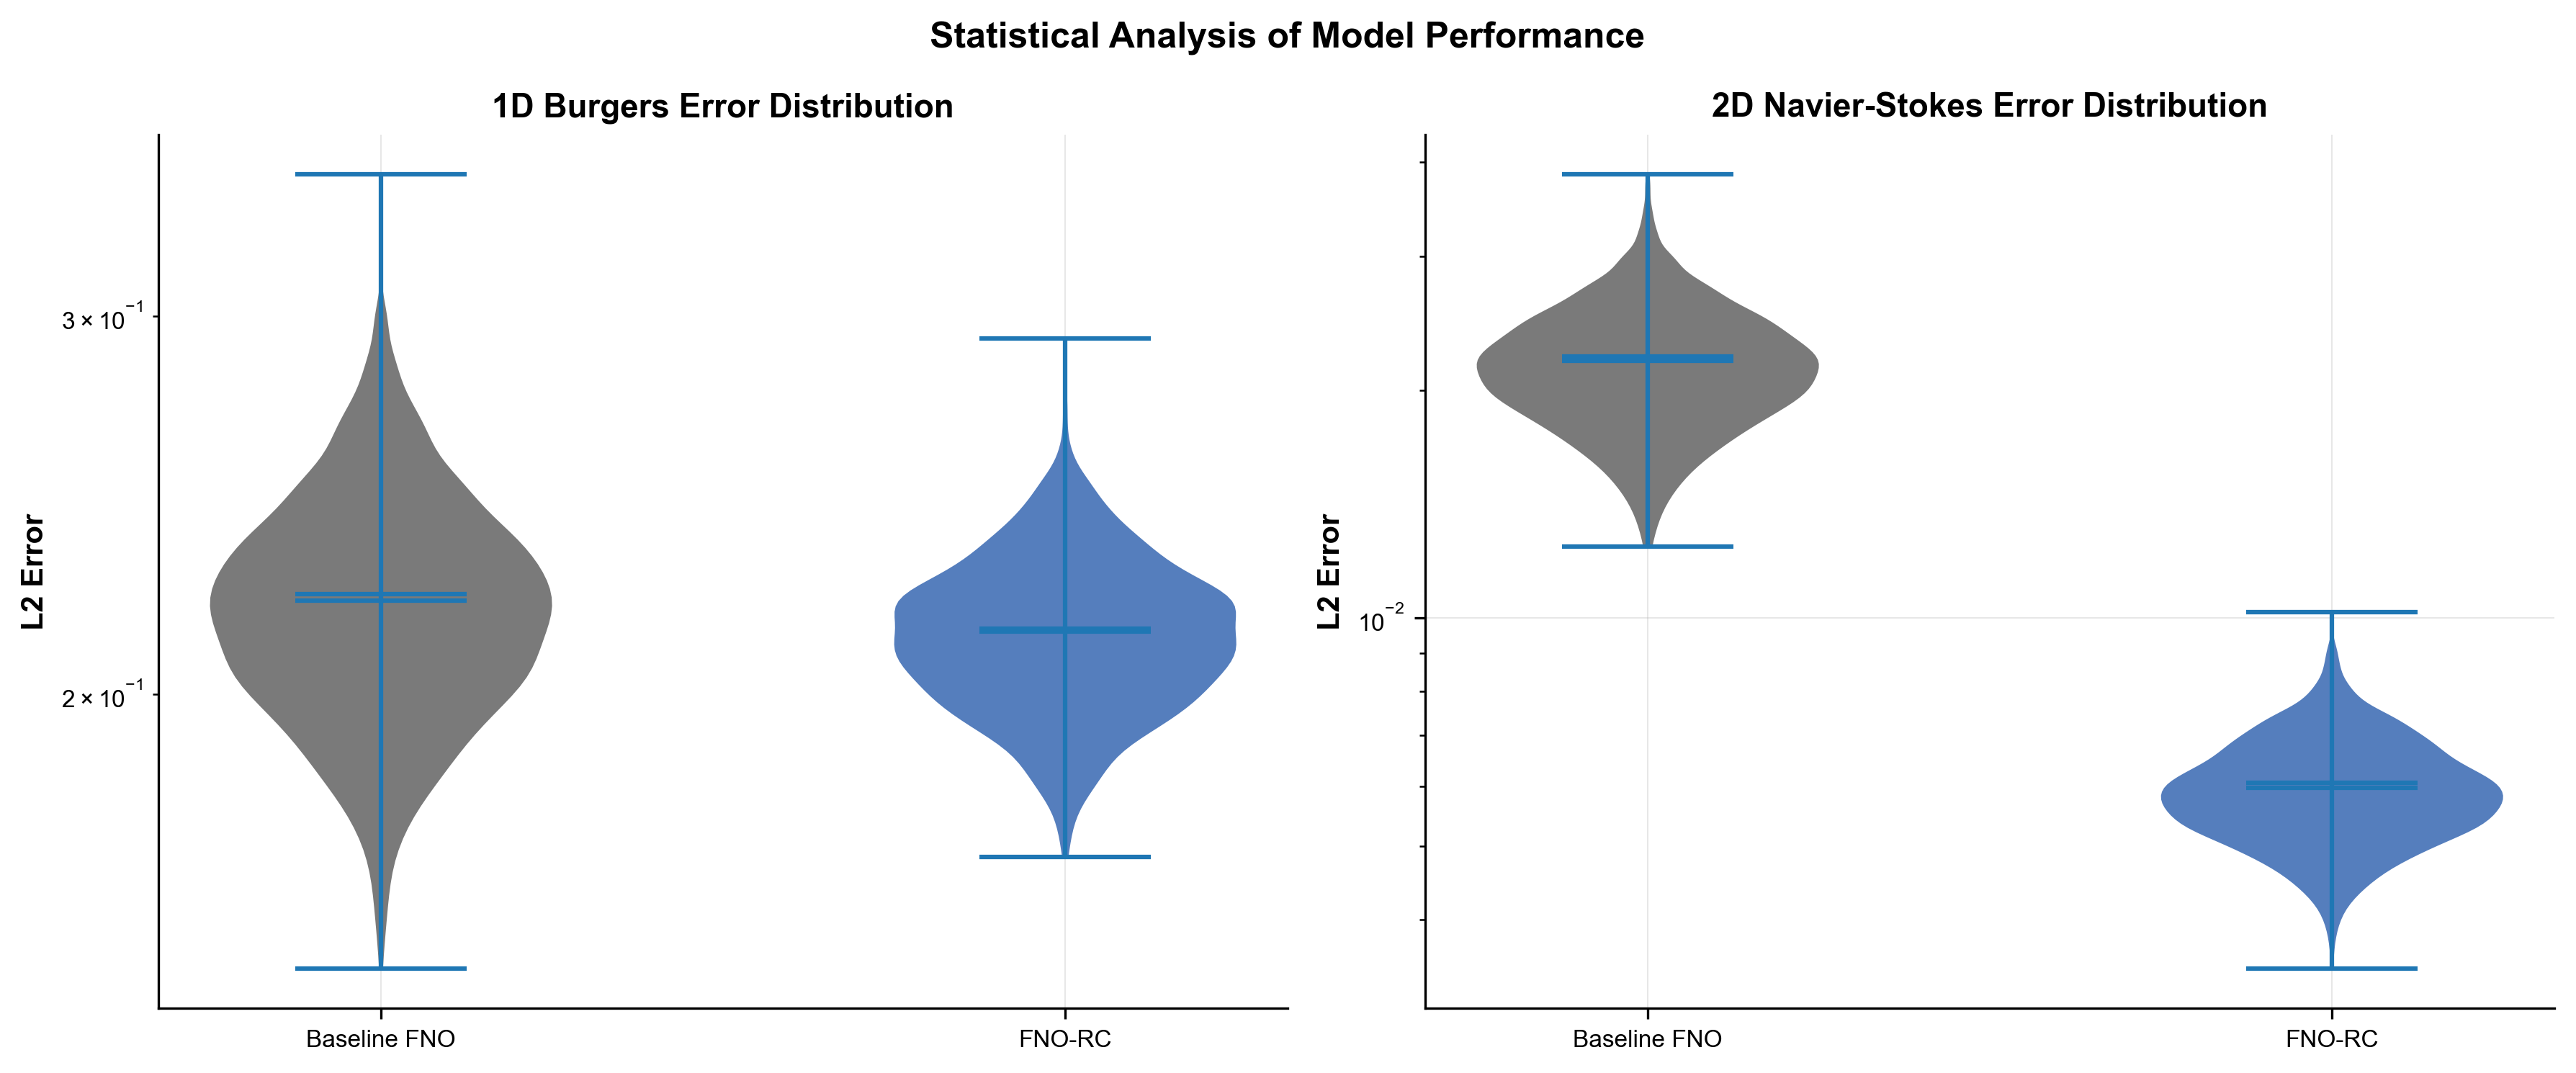
\includegraphics[width=.95\linewidth]{figures/long_term_prediction.png}
  \caption{Long-horizon rollouts ($H{=}100$). FNO-RC reduces autoregressive error accumulation.}
  \label{fig:rollout}
\end{figure}

\begin{figure}[t]
  \centering
  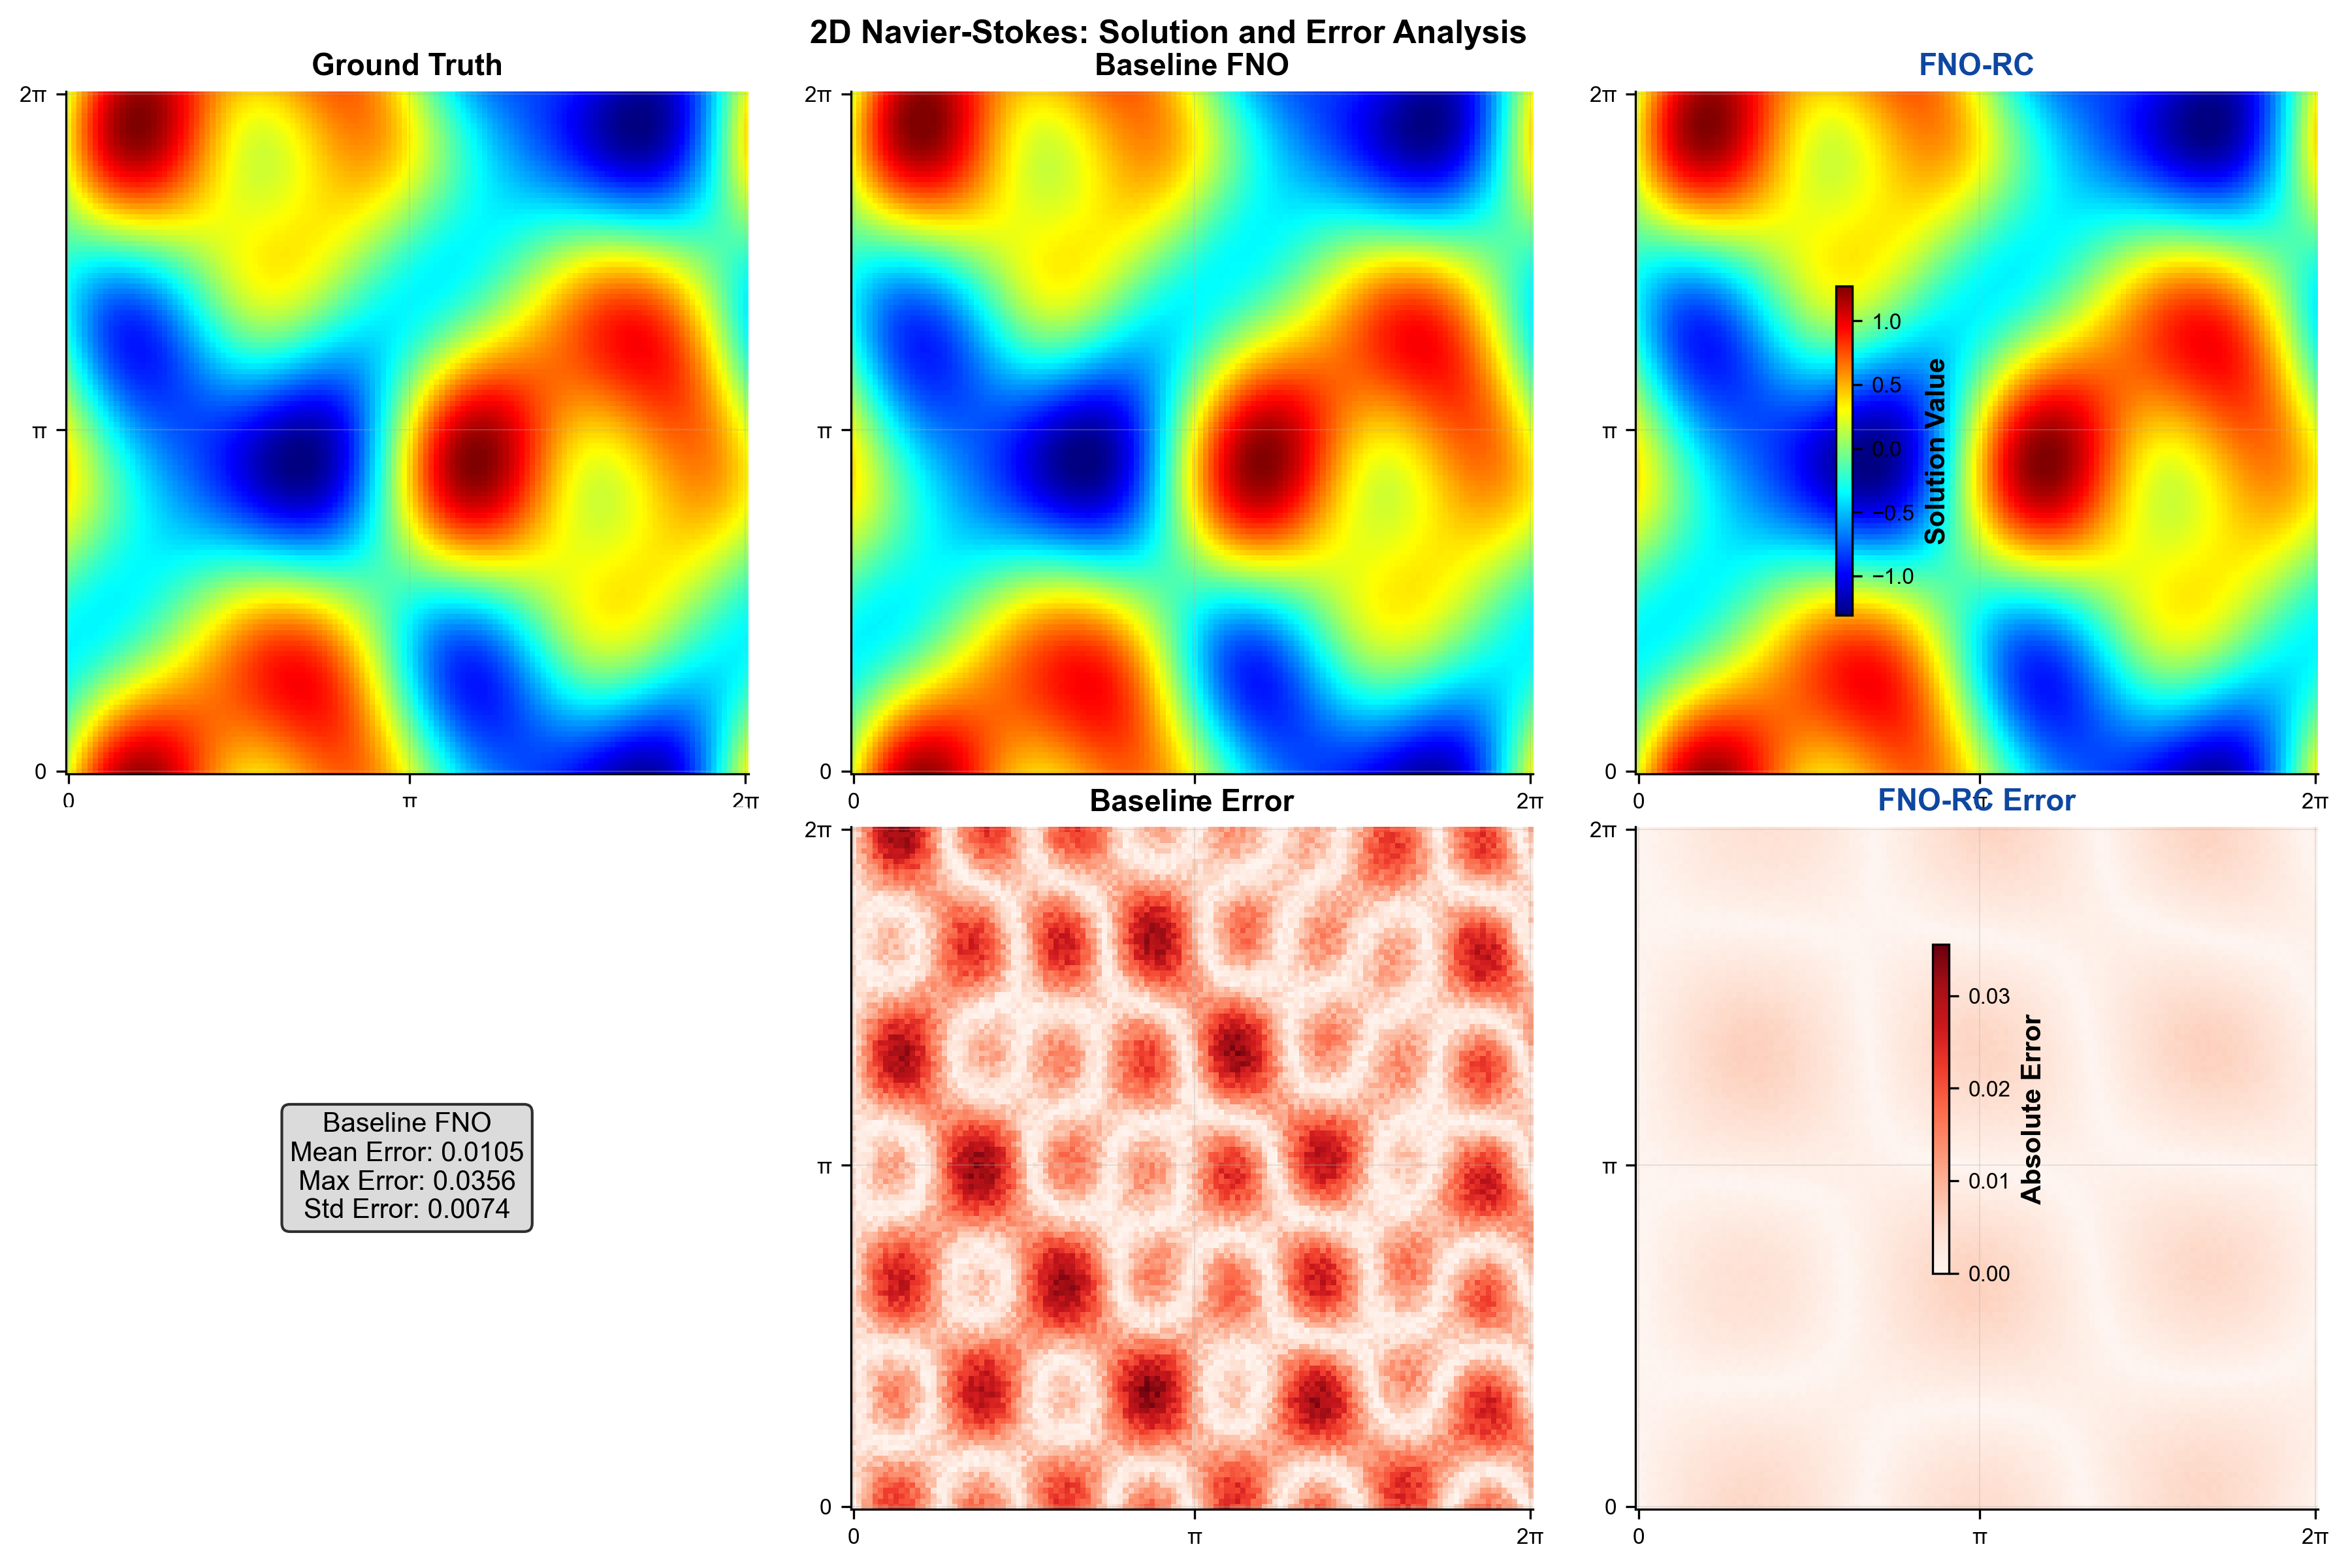
\includegraphics[width=.95\linewidth]{figures/error_analysis.png}
  \caption{Spectral/error diagnostics (energy spectra, amplitude/phase errors).}
  \label{fig:spectrum}
\end{figure}

\begin{figure}[t]
  \centering
  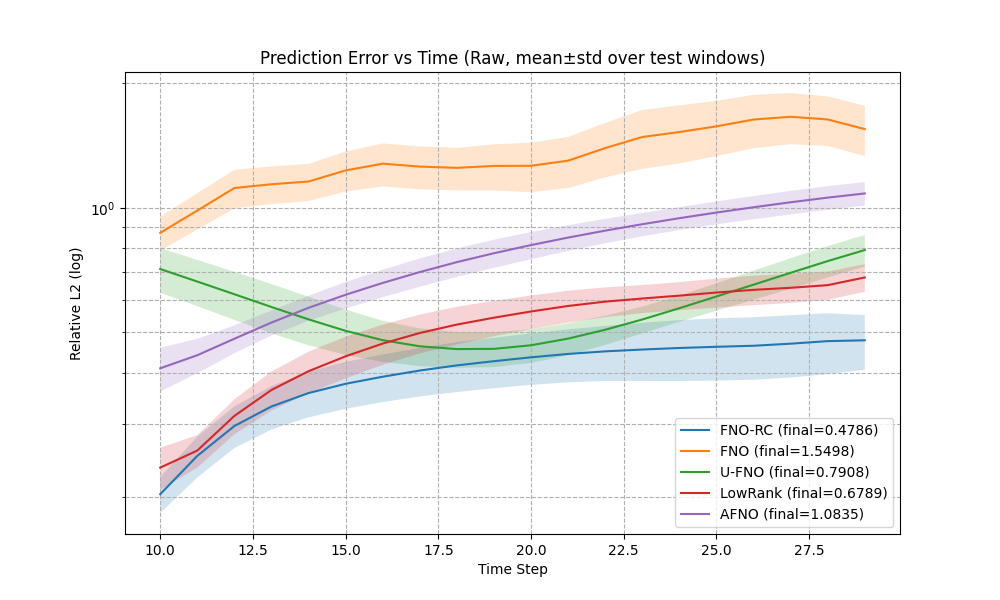
\includegraphics[width=.95\linewidth]{../实验图/error_vs_time_raw_mean.png}
  \caption{Error vs time (raw mean) on 3D tasks.}
  \label{fig:error_time_raw}
\end{figure}

\begin{figure}[t]
  \centering
  \begin{subfigure}{.49\linewidth}
    \centering
    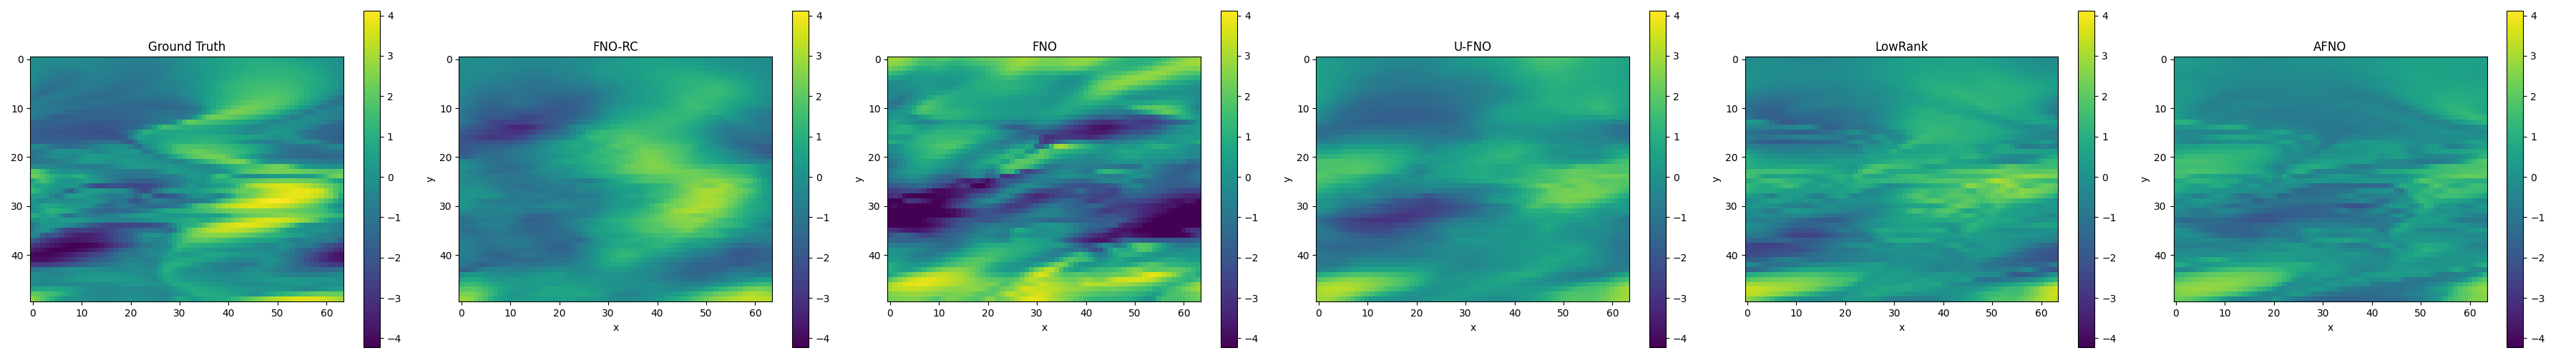
\includegraphics[width=\linewidth]{../实验图/final_slice.png}
    \caption{Final slice}
  \end{subfigure}\hfill
  \begin{subfigure}{.49\linewidth}
    \centering
    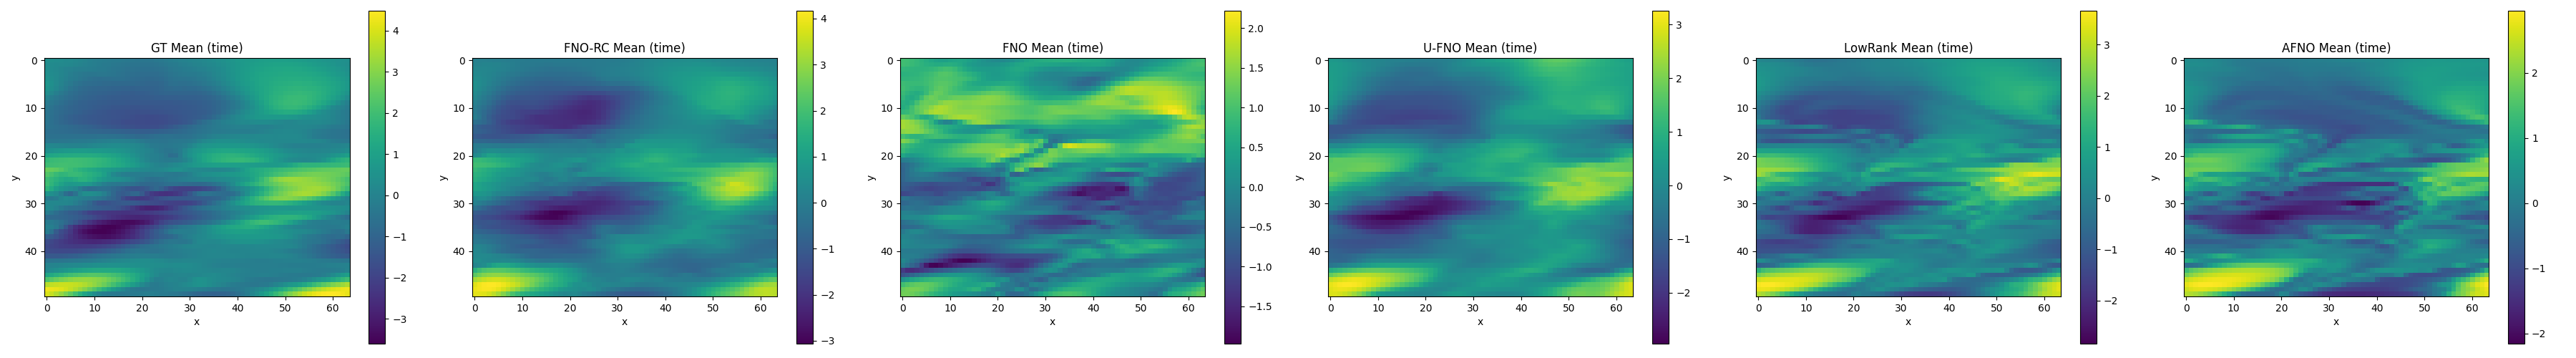
\includegraphics[width=\linewidth]{../实验图/mean_time.png}
    \caption{Time-mean}
  \end{subfigure}
  \caption{Qualitative comparisons on 3D fields.}
  \label{fig:qualitative}
\end{figure}

\section{Discussion}
Residual correction improves temporal stability; conservative use (shallow RC, small initial $\gamma$) with HF regularization addresses high-$k$ shift under resolution changes.

\section{Conclusion}
FNO-RC integrates continuous Fourier features as a conservative residual atop FNO, achieving improved long-horizon stability with competitive cross-resolution performance.

\bibliographystyle{plainnat}
\bibliography{references}

\end{document}


